\chapter{Background}\label{background-chapter}
This chapter will introduce the theoretical background of this thesis. We start with a high-level discussion of virtualization, which forms the basis of container-based virtualization and cloud-based IDEs such as CodeExpert. We close this chapter by introducing the Nix build system.

\section{Virtualization}
Virtualization is one of the most fundamental ideas in computer science, and many components of a computing system`s software, hardware, and network use it. It has become prevalent and is used by many developers and organizations for cloud computing, security, testing, and development.

\emph{Virtualization} is commonly defined as a technology that introduces a software abstraction layer between the hardware and the operating system and applications running on top of it. This abstraction layer, called virtual machine manager (VMM) or hypervisor, hides the physical hardware resources from the operating system (OS). This means that an application program cannot differentiate between a virtual and a real execution environment, but the abstraction layer allows the underlying mechanisms to differ. Since the VMM, not the OS, controls the hardware resources, they can be partitioned into several logical units called virtual machines (VM) to allow running multiple OSs in parallel \cite{Sahoo2010}.  

The two primary advantages of virtualization are generally \emph{resource sharing} and \emph{isolation}. The former is the ability of a virtualized environment to share resources (i.e., memory, disk, and network devices) of the underlying host. For virtualization, it is essential to provide isolation between VMs running on the same hardware.
%The term ``virtual machine'' in the sense of ``abstract machines'' is used to describe highly abstract execution environments, such as the byte code executed by the Java Virtual Machine \cite{alma990050088570205503}. We restrict ourselves to the discussion of virtual machines (VM) that provide a simulation of raw machine hardware as the execution environment. This means that the applications run in this environment are operating systems in this thesis. 

\subsection{The uses of VMs}
This section briefly covers the essential use cases of VMs, where the use case of cloud technologies is described in more detail since it is important for this thesis.

\paragraph{Important use cases of VMs}
Programmers use VMs to ease software development and testing. Furthermore, they are used in \emph{cloud computing} that enables access to a shared pool of computing resources that can be provisioned and released with minimal management effort \cite{Mell2011}. In cloud computing, hypervisors decouple the allocation of resources (VMs) from infrastructure provisioning (physical machines). VMs provide \emph{resource isolation}, which is the property of an OS guaranteeing to one application that others will not impact its performance. The OS does not guarantee resource isolation, as it lacks resource containers \cite{Banga1999}. The OS can sometimes perform resource isolation between processes, but applications comprise many processes, and multiple applications share many processes. Thus when multiple applications content for resources (CPU time, physical memory), the performance of one or more may degrade in ways outside the control of the OS. 

\paragraph{Cloud technologies}
Cloud technologies achieve, among others, the following attributes: rapid elasticity and resilience \cite{Mell2011}. Resilience refers to handling failure, whereas elasticity is the ability to request more resources on demand. Cloud technology is usually split into two components: infrastructure and services, where, e.g., Docker provides both the infrastructure and platform to host services. Software running as a service is \emph{cloud native} if built from the very first steps to run inside the cloud. Cloud-native applications are generally run inside a container and are resilient and elastic by design \cite{Applis2019}\cite{TOFFETTI2017165}.

\subsection{Hypervisor-based virtualization}
There is commonly a distinction between a VMM and a hypervisor. A VMM is a functionality required to create the illusion of real hardware for a single \emph{guest OS}. Specifically, a VMM creates a \emph{single} virtual machine. A guest operating system is an OS, plus associated applications, running inside a virtual machine. On the other hand, a hypervisor is software that runs on actual, physical hardware and supports \emph{multiple} virtual machines -- each with its associated VMM. A hypervisor is usually an operating system and is required to create and run VMs. A hypervisor-based virtualization system can be of two types: \emph{hardware-layer virtualization} or \emph{type 1} and \emph{type 2} hypervisors (see figure \ref{fig:Virtualization}). 

In hardware-layer virtualization, the hypervisor runs ``on the metal'', i.e., it runs directly on the hardware layer as an OS kernel, controlling and synchronizing the access of the guest OS to the hardware resources. A VM is represented by a guest OS, which can differ across VMs, libraries, and applications. Figure \ref{fig:Hypervisor-type-1} depicts this architecture. It is commonly used due to its high isolation and performance of VMs \cite{Sahoo2010}. IBM VM/CMS, VMware ESX, and Xen are examples of type 1 hypervisors.

Type 2 hypervisors run on top of or as part of the host OS, commonly as an application in \emph{user-space}. The result is that in each VM, the application and the guest OS run on top of the virtual hardware provided by the VMM (see fig. \ref{fig:Hypervisor-type-2}). As with type 1 hypervisors, each VM requires a full copy of the guest OS, applications, and libraries \cite{Sahoo2010}. The user-space is a set of memory locations normal user processes can access. It is distinct from the kernel space, which the kernel can only access. %Depending on the hypervisor's implementation, the guest OS is run without modification to provide ``Full Virtualization'' or modified in ``Para-virtualization''. The modified guest OS is usually ``aware'' that it runs inside a virtualized environment. Full virtualization is easier to use as an ordinary user can install any guest OS on a chosen type 2 hypervisor. On the other hand, para-virtualization allows for a simpler hypervisor and usually achieves better performance \cite{Sahoo2010}. 
VMware Workstation, KVM, and VirtualBox are all examples of type 2 hypervisors.

\begin{figure}
\begin{subfigure}[t]{0.49\textwidth}
\centering

\includegraphics[width=\textwidth]{thesis/graphics/hardware-layer-virtualization.png} 
\caption{Hardware-layer virtualization or type 1 hypervisor}
\label{fig:Hypervisor-type-1}
\end{subfigure}
\begin{subfigure}[t]{0.49\textwidth}
\centering

\includegraphics[width=\textwidth]{thesis/graphics/full-virtualization.png}
\caption{Full virtualization or type 2 hypervisor}
\label{fig:Hypervisor-type-2}
\end{subfigure}

\caption{Different types of hypervisor-based virtualization architectures (adapted from \cite{Sahoo2010}).}
\label{fig:Virtualization}
\end{figure}

\subsection{Container-based OS-layer virtualization}\label{OS-layer-virtualization}
Containers share some characteristics with VMs but are an example of \emph{OS-level virtualization}. OS-level virtualization, represented by the \emph{virtualization layer} -- also known as \emph{container engine}, virtualizes a single host OS to provide the illusion of multiple instances or ``containers'' of that same OS (see fig. \ref{fig:OS-Layer-virtualization}). Unlike hypervisors, each container is constrained to run the same OS as the host. This means that the host’s kernel is shared, and applications can safely share system libraries and executables across containers rather than having possibly redundant copies in each VM. Multiple containers can be run in parallel, and each can be started, stopped, and removed by the container engine. The ability of containers to share resources with the host OS and share data with other containers makes them efficient \cite{Mouat99117185791205503}\cite{redHatContainerTerms}. 
%Containers are an encapsulation of an application with its dependencies.

OS-level virtualization achieves isolation by limiting the \emph{filesystem namespace} and the \emph{process namespace}. The process namespace binds a process to its execution environment. The filesystem namespace refers to the organization of the bindings between names and files. The filesystem namespace can be limited by changing the root for each container. The process namespace is limited, so processes can only ``see'' other processes that share their container. The OS or virtualization layer may provide more sophisticated scheduling and memory allocation policies for running containers instead of standard processes. How this is done exactly is out of the scope of this thesis. 

A privileged container (see fig \ref{fig:OS-Layer-virtualization}) exists in this system that provides an interface to the virtualization layer. This allows a system administrator to manage other containers and assign resources to containers at the time of creation or dynamically at runtime. These resources could include disk space, CPU guarantees, and memory limits. To applications and the user of a container-based system, the container appears just like a separate host. Processes running inside the container are native processes on the host with the same system call interface as the underlying host OS \cite{Soltesz2007}\cite{Mouat99117185791205503}. 
\begin{figure}
  \centering
  
\includegraphics[width=0.7\textwidth]{thesis/graphics/OS-layer-virtualization.png}
  \caption{OS-Layer virtualization architecture overview as the basis of containers (adapted from \cite{Sahoo2010}).}
  \label{fig:OS-Layer-virtualization}
\end{figure}

\subsection{Containers versus VMs}\label{containers-vs-VM}
Containers and VMs can both be used to isolate applications from each other running on the same hardware. They are commonly used to achieve different goals -- containers are used to make applications \emph{self-contained} and \emph{portable}, while the purpose of VMs is to emulate a system entirely. Self-contained means that the application does not rely on dependencies external to the container. Portability is hiding the details of an application's execution environment to transfer it to another platform effortlessly. A platform includes hardware, the OS, system users, and software interfaces. Containers are somewhat limited in functionality compared with VMs, but they enable use cases that are difficult to achieve with VMs \cite{Mouat99117185791205503}. 

The self-containment and portability properties of containers have advantages in cloud deployment and for developers who can download images and run containers without worrying about configuration, differences in user environments, and installing dependencies \cite{Mouat99117185791205503}. Containers can be started and stopped in a fraction of a second. Processes of containers do not incur the overheads of hypervisor execution (e.g., interpreting system calls). The sharing property of a container system makes containers more efficient (``lightweight'') compared to VMs. This results in system administrators being able to run many more containers on a single host machine than VMs. 

Research confirms the above claim that containers tend to be more efficient and suggests that they guarantee almost the same resource isolation as VMs (at present; some researchers dispute both claims) \cite{Soltesz2007}. However, hypervisors are a trusted and battle-tested technology, whereas containers are comparatively new, resulting in companies not fully trusting the isolation of containers. This lack of trust has led to hybrid systems with containers running inside VMs to take advantage of both technologies \cite{Mouat99117185791205503}. 

\section{Containers}
Containers are an old idea, where a basic form of system-level virtualization was introduced to FreeBSD in 1998. Then in 2008, the Linux Containers project (LXC) started and brought together system-level virtualization and resource limiting for memory and CPU. The result was a complete containerization solution. The final piece to the containerization ecosystem was brought by Docker in 2013 and enabled widespread adoption of the technology by companies like Red Hat, Microsoft, and Amazon and the developer community. Docker extended existing Linux container technology (i.e., LXC) with a standard container format to allow portable images. It also added a user-friendly interface and tools to build, run and distribute containers \cite{Mouat99117185791205503}. 

The different available container solutions, each having a different container image format, and the rise of Docker led to the development of an independent formal standard for the container runtime and image format. This standard is known as \emph{OCI Image Specification} after the governance structure Open Container Initiative (OCI) that created it. The OCI Image Specification was based on the original Docker image format and is adopted today by almost all major container engines and tools. LXC and many other container engines and container orchestration options exist, such as OpenVZ and Kubernetes, but Docker remains the industry standard containerization software \cite{Mouat99117185791205503}. 

This section introduces essential concepts of a container system used in this thesis. The theoretical and abstract view of such a system was introduced in \ref{OS-layer-virtualization}  Since the current CodeExpert approach and our prototypes use Docker, we will use it in the following as an example for some of the more general containerization concepts.

\subsection{Container image}\label{container-image}
%When we use the term \emph{container image} in this thesis, we mean images in the OCI image format. This format defines a container image as a collection of multiple tar files (one file for each \emph{layer}) and a \emph{configuration file} \cite{redHatContainerTerms}. 
Container images are already introduced in definition \ref{def:container-image}. %The configuration file contains image metadata, which provides extra information about the layers, and an ordered list of layer references -- not the actual files of each layer \cite{BraunDockerLayers}.
An image often extends another image, called the \emph{base image}, with some additional customization, i.e., software packages necessary for running one's application. Images are then used to store one's application and deploy it to a server. In the case of Docker, the instructions defining the steps needed to build the image and run it are written with a \verb|Dockerfile| \cite{dockerOverview}.

\subsection{Container}\label{containers}
%A \emph{container} has two states (resting and running), similar to the states of a process. In the rest state, it is a set of files and metadata (i.e., the container image) saved on a disk. When one starts a container, the container engine creates a runtime instantiation of the container image. In particular, the container engine unpacks the set of files and metadata and makes a system call to the kernel to start a process. This system call initiates extra isolation (see \ref{OS-layer-virtualization}) and mounts (i.e., makes available to users) a copy of the container image files. Now the container is in the running state as a Linux process. 
A container has been defined in \ref{def:container}, and some other important properties are introduced next. Typically, configuration options can be added to a container when starting it, like limiting the memory capacity or setting environment variables. Thus a running container is defined by the container image used as a mount point to start it and the provided configuration options \cite{redHatContainerTerms}. One can connect a container to subsystems such as network or persistent storage (introduced in \ref{container-storage}) and control the degree of isolation of each container from other containers and the host machine. The container life-cycle ends when removing a stopped container and any state not stored in persistent storage or the image's layers at build time disappears \cite{dockerOverview}. 

\subsection{Image layers}\label{layers}
We need to know how layers are created, stored, and cached to understand the uses and performance aspects of images and containers. In this section, we will use Docker as an example to explain the relation between images and layers and the connection between containers and layers.

\paragraph{Images and layers}\label{images-and-layers}
Recall from definition \ref{def:container-image} that container images are a collection of layers. Layers in an image relate to each other through a parent-child relationship. The union of all layers comprises the content of an image. Each image layer represents the changes between itself and the parent layer. Each parent layer contains the set of differences (\verb|diff|) to the filesystem of the child layer. %In the case of Docker, the instructions in a \verb|Dockerfile| specify how an image is built. %All other instructions in a \verb|Dockerfile| only change the image's metadata and do not produce a new layer. 
For example, in the case of Docker, if a \verb|Dockerfile| instruction copies a file into the image's filesystem, this file is located in the \verb|diff| of a layer \cite{DockerStorageDrivers}\cite{BraunDockerLayers}. Each layer is identified by a \emph{content addressable ID} that is the hash value of its content \cite{BraunDockerLayers}. A content addressable store is analogous to the concept of \emph{content addressable memory} that `refers to a principle of organization and/or management of memories [...], or searching of data on the basis of their contents rather than by their location \cite[p.~1]{Kohonen1980}.' The modifications of the \verb|Dockerfile| that result in changes of the \verb|diff| of a layer are cached as a separate layer cache. A container image is built by progressively merging the files inside the layers on top of the base image. The cached layer is used whenever possible during the merging. The merging of layers is possible due to the \emph{union filesystem} that Docker uses that allows stacking multiple filesystems or directories to appear as a single filesystem \cite{DockerStorageDrivers}\cite{Wright2004}.

The two primary advantages of constructing images and layers in this format are efficient storage usage and faster rebuilds. The separation of the image configuration file from the files that store the contents of the layers allows sharing layers among multiple image configurations by referencing the same layer. Thus, for example, if multiple images use the same base image, then the layers of the base image have to be stored only once on disk resulting in efficient disk usage \cite{DockerStorageDrivers}.
The cached layers avoid recomputations in an image rebuild after a configuration change. Specifically, almost only those changed layers are rebuilt, resulting in faster image builds \cite{dockerOverview}.
%In the case of Docker, each layer has its own directory within Docker's storage directory that contains, among others, the \verb|diff| and the \verb|cache-id|. Each layer has an associated cache, which is identified by the hash value of the cache (the \verb|cache-id|). Just as with layers, Docker stores all cached layers in directories that correspond to the cache ID. Cache directories contain a subdirectory called \verb|diff|, representing the modification to the filesystem \cite{BraunDockerLayers}. 

\paragraph{Containers and layers}\label{containers-and-layers}
When a new container is started, a new writable layer is added on top of the read-only layers. This writable layer is the significant difference between a container and an image and is why it is often called the ``container'' layer. This layer allows some write access to containers, as all changes made to the running container, such as writing, modifying, or deleting files, are written to this thin container layer. To achieve this, Docker utilizes a \emph{copy-on-write} mechanism that copies a file from some read-only layer to the writable layer if the container updates the file for the first time. This mechanism implies that containers that write a lot of data, which the copy-on-write mechanism writes to the writable layer, consume more space than those that do not. When a container is deleted, the writable layer disappears, and the underlying image remains unchanged \cite{DockerStorageDrivers}. The copy-on-write mechanism helps to make containers efficient. It saves space, as the read-only layers can be shared among containers. Additionally, it reduces container start-up time, as the container engine only needs to create the container layer \cite{DockerStorageDrivers}.
\begin{figure}[h!]
  \centering
  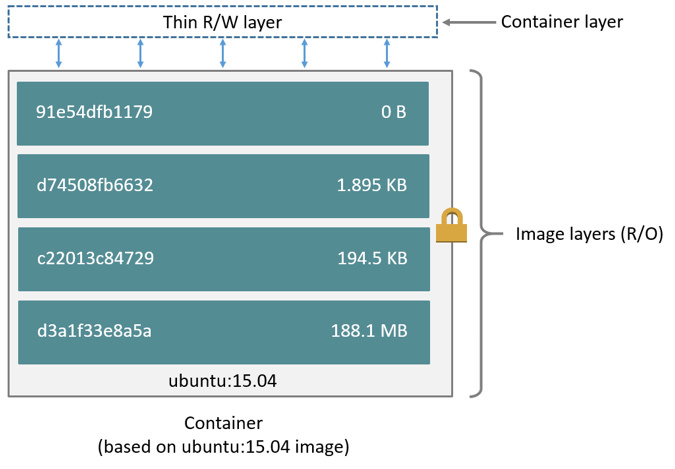
\includegraphics[width=\textwidth]{thesis/graphics/container-layers.jpg}
  \caption{Docker container layers based on ubuntu:15.04 image. R/W means that the container can read and write to this layer. Each read-only (R/O) layer is represented by its content-addressable hash and size of the layer \cite{DockerStorageDrivers}.}
  \label{fig:container-layers}
\end{figure}

\subsection{Image registry}
A \emph{image registry} is a repository, typically run as a server, for storing images. If the container engine does not have a locally cached copy of the container image, it will automatically try to download (``pull'') it from an image registry server. It is also possible to upload (``push'') a locally built image to an image registry. One can configure the registries the container engine will use to pull images from -- Docker uses, by default, the public registry called Docker Hub. It is also possible to run a private registry instance for example in a container \cite{dockerOverview}\cite{redHatContainerTerms}. 

\subsection{Storage}\label{container-storage}
The following section provides an overview of standard persistent storage options that can be attached as a subsystem to a container. For this section, we use the documentation of Docker, but the different storage types apply to other containerization options. Our prototype uses some introduced storage options to persist data across the container life-cycle. 

This thesis uses two storage types: volumes and bind-mounts. We can visualize their differences by looking at where the data is stored on the host machine (see figure \ref{fig:docker-storage-overview}). Another common storage type (tmpfs mounts) is out of the scope of this work.
\begin{figure}[h!]
  \centering
  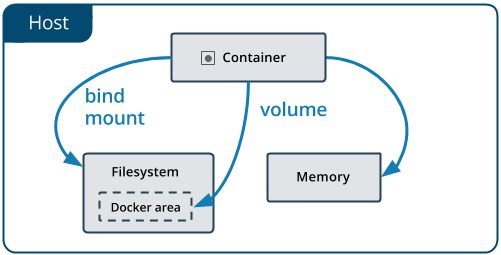
\includegraphics[width=0.7\textwidth]{thesis/graphics/types-of-mounts.png}
  \caption{Location of where the data of volumes and bind mounts is stored on the host machine (adapted from \cite{DockerStorage}).}
  \label{fig:docker-storage-overview}
\end{figure}
\paragraph{Volumes}
\emph{Volumes} facilitate persistent data storage that can be shared safely across multiple containers. New volumes can have their content prepopulated by a container. Volumes are often chosen over persisting data in a containers writable layer (see \ref{containers-and-layers}). The reason is that a volume does not increase the size of the containers using it and the data stored in the volume exists outside the life-cycle of a container. In the case of Docker, a volume is stored in a directory within Docker`s storage directory on the host machine, and Docker manages a volume by managing that directory`s contents (see fig. \ref{fig:docker-storage-overview}) \cite{DockerVolumes}\cite{DockerBindMounts}. 
\paragraph{Bind mounts}
When using a \emph{bind mount}, a file or directory -- specified by an absolute path -- on the host machine is mounted into a container. The bind mounts may be stored anywhere in the filesystem of the host and can be modified by processes inside the container and on the host (see fig. \ref{fig:docker-storage-overview}) \cite{DockerStorage}. Bind mounts have limited functionality and are much less performant on Windows or Mac hosts compared to volumes \cite{DockerBindMounts}\cite{DockerVolumes}. Nonetheless, they help mount a small number of specific files into a container and are very performant on Linux hosts, provided that the host has the right filesystem directory structure \cite{DockerBindMounts}.
%\paragraph{tmpfs mounts}
%This storage option is useful to temporarily store sensitive files that one does not want to store in the host filesystem or the container's writable layer. Unlike bind mounts or volumes, a \verb|tmpfs| mounts are temporary and persist data in the host memory (see fig. \ref{fig:docker-storage-overview}). Once the container stops, the \verb|tmpfs| mount is removed, and the files written in the mounts memory area are deleted \cite{DockerTmpfsMount}. 

The containerization concepts from this chapter and the virtualization chapter form the basis for the next chapter on cloud-based integrated development environments that often use containers to execute users' code remotely.

\section{Cloud-based integrated development environments}\label{cloud-based-IDE}
This section introduces cloud-based IDEs and their difference from traditional IDEs. Additionally, we cover the implications of a cloud-based IDE on how a programming environment should be set up.

Traditional Integrated Development Environments (IDEs) accelerate software development by providing an effective way to browse and manipulate a system's source code as opposed to using a plain text editor and command line \cite{BruchBodden2010} \cite{FYLAKTOPOULOS2018127}. A traditional IDE provides developers with a development environment where the IDE is commonly responsible for tasks such as dependency management, debugging, and auto-completion \cite{Applis2019}. Popular IDEs include Microsoft Visual Studio, Eclipse, and NetBeans.

A cloud-based IDE is run in a cloud computing system, and developers can access the IDE from any web browser at any time \cite{Yanagisawa6354897}. Compared to a traditional IDE, which must be installed before using it, each developer does not have to install dependencies and compilers on the local system. Cloud IDEs set up a shared workspace, which is shared among the programmers. Furthermore, they provide a large pool of computing resources for development to support developer collaboration. Popular cloud-based IDEs include CodeSpaces, Cloud9, Replit, and Eclipse Che. 

A cloud IDE should offer programming languages as runtime execution environments as developers may want to use different programming languages. These environments are often executed inside containers, making them cloud-native applications. Furthermore, a standard runtime environment configuration can be shared among developers \cite{Applis2019}\cite{FYLAKTOPOULOS2018127}.

\section{CodeExpert}\label{CodeExpert}
Since this thesis compares its results to the current implementation of \emph{CodeExpert} and discusses its tradeoffs, we need to understand its architecture and general workflow.

\subsection{Architecture}
CodeExpert is a cloud-based IDE developed at ETH Zürich that is used to enhance computer science studies and programming classes. The architecture consists of four primary services, split into the front-end (\emph{cxweb}) and the back-end. The back-end includes the database, back-end runner (\emph{cxrun}), and image registry (see fig. \ref{fig:cx-architecture}). The CodeExpert IDE is accessed via web browser and executed inside containers.
\begin{figure}
   \centering
   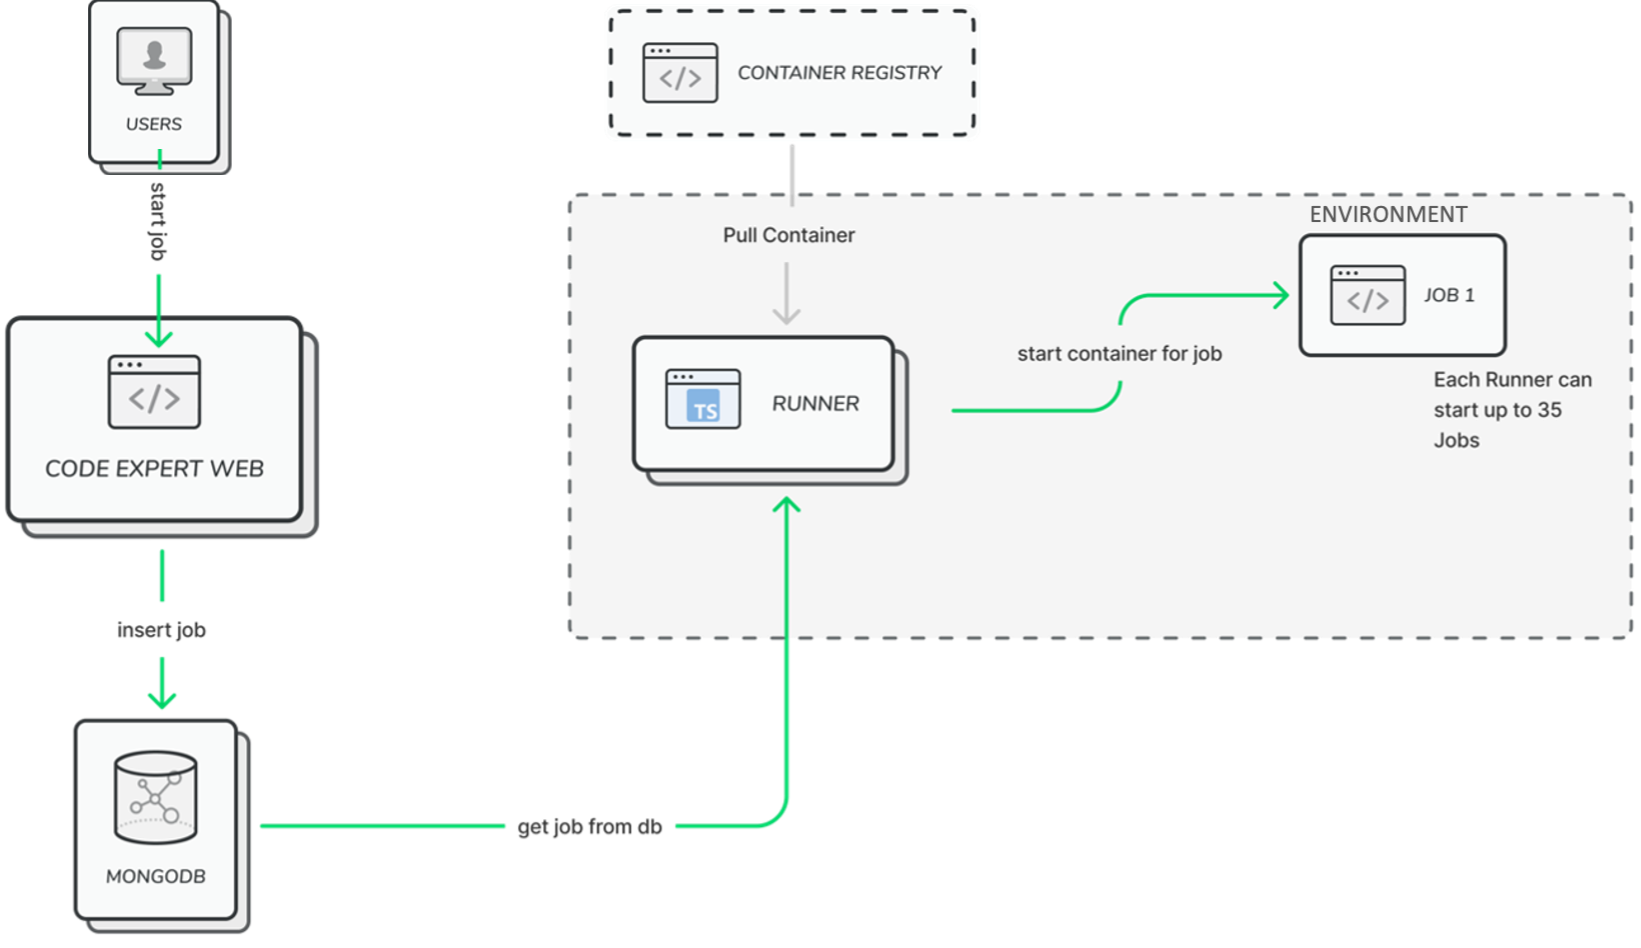
\includegraphics[width=\textwidth]{thesis/graphics/CodeExpertArchitecture.png}
   \caption{CodeExpert architecture and job execution flow (adapted from \cite{CodeExpertTechnicalOverview})} 
   \label{fig:cx-architecture}
\end{figure}
The front-end is separated from the back-end through interfaces. Each service is running on multiple different virtual machines. This decoupling of the front-end from the back-end allows the system to scale -- as the workload increases -- the back-end and front-end services independently. 

\subsection{Execution flow}\label{CX-execution-flow}
For each interaction (e.g., executing or compiling code) of the student, cxrun starts a new cloud-native environment (\emph{cxEnvironment}) in which the code is executed remotely. After the execution has terminated, the container is removed, and the execution output is redirected by cxrun to cxweb. This allows the student to inspect the output \cite{CXDocs}. 

\subsection{Configuration}\label{CX-configuration}
The lecturer explicitly specifies the cxEnvironment for each project, and the lecturer can use predefined cxEnvironments for programming languages such as \verb|C|/\verb|C++|, \verb|Python|, and \verb|Java|. Lecturers can also define a custom cxEnvironment using a \verb|Dockerfile|, which is then built to an image and pushed to the image registry (denoted as ``container registry'' in fig. \ref{fig:cx-architecture}). The image registry runs in a container inside the local network. The building and pushing are done at build time before the custom image can be used as runtime environment \cite{CXDocs}.

\section{Build system}
After our discussion on cloud-based IDEs and CodeExpert, this section will introduce some properties and tools of a \emph{build system} that we will use to build images at runtime. 

\subsection{Reproducibility}\label{reproducibility}
Coding environments that lectures use for their student should be \emph{reproducible}, as they are, for example, used in exams. Reproducibility of environments means building the same configuration twice should yield the same environment. To achieve reproducibility, we must manage software versions and dependencies and manage development environments. The latter is commonly handled with containers (e.g., Docker) and VMs that provide controlled environments in which the user code can be executed \cite{bedo2010}. 

We have already learned that a container image allows reproducible containers (see definition \ref{def:container}). However, the Docker image build system does not guarantee reproducible images. When building images twice from the same \verb|Dockerfile|, one might get two images that behave differently. The different behaving images could break the user's runtime environment. This non-determinism happens, for example, when a third-party package dependency gets silently updated or when the package version is not specified (``pinned'') when writing the \verb|Dockerfile|. The silent update results from non-purely-functional package managers (a concept explained in \ref{Nix-theory}), whereas not pinning the package version is a terrible practice. Pinning all package versions helps, but there are many details to consider, and it does not relieve the issue completely \cite{OHearn}.

The non-reproducibility issues of building images with \verb|Dockerfile|'s motivate the use of a purely functional package manager and a system to build the coding environment, called a \emph{hermetic} build system. Given the same input source code and configuration, this system returns the same output using isolation and \emph{source identity}. This is the topic of the next section.

\subsection{Hermeticity}\label{hermeticity}
A \emph{hermetic} build system isolates the build from the underlying host system. Thus a hermetic build is insensitive to libraries and software installed on the host machine and depends only on specific versions of build tools (e.g., compilers) and dependencies (e.g., libraries). The result is self-contained builds \cite{HermeticityBazel}. 

A hermetic build tries to ensure the consistency and sameness of inputs, a concept called source identity. Source identity is achieved with the help of code repositories, such as Git, where the unique hash code that identifies code mutations is used to track changes to the build's input. More specifically, isolation between the host machine and the user is achieved by downloading copies of tools and managing their storage inside managed file trees \cite{HermeticityBazel}. 

The benefits of having a hermetic build system are speed, multiple parallel builds, and having multiple versions of the same package coexist. Builds can be cached unless the inputs change, resulting in fast builds. Parallel builds can be executed by computing the graph of actions to take such that the output is built from the input. As the storage of the packages is managed by the hermetic system, we can easily use different versions of tools in multiple builds without colliding installation paths. Thus, we do not need to create a different container environment for different package versions \cite{HermeticityBazel}\cite{NixPills1}. Furthermore, a hermetic build system implies reproducibility \cite{HermeticityBazel}. Since the build output does not depend on anything outside the build, we can copy it across different systems and potentially make it portable.

\subsection{Package manager}
Software platforms strive to provide modular software components, called software \emph{packages} that can be assembled to provide the user with the desired functionalities. A package is an archive file containing a program and necessary metadata. The program can be in \emph{source code} that must be compiled and built first. The metadata may include, among others, the package version and description and requirements for relationships (e.g., versions) to other packages and the target system. Installing more than one copy of a package on a given system is impossible. Packages cannot be composed to build a larger component, and they may conflict with each other. The latter can happen because the installation and execution of packages act on shared resources provided by the OS, like creating files or interacting through the systems input/output devices. The essential tools for managing software versions and their dependencies (installing, upgrading, and removing packages) are \emph{package managers}. They allow to retrieve packages from central (remote) repositories and check their integrity. Furthermore, they resolve conflicts between package requirements and provide tools to manage the installation on a user's system. Resolving requirements conflicts is a functionality known as \emph{dependency solving} and is introduced next \cite{ABATE2013459}\cite{bedo2010}. 

\subsection{Dependency management}
\emph{Dependency management} is usually specific to your OS, programming language, or application and is either done by an IDE (see \ref{cloud-based-IDE}) or by a separate package manager. Some examples of popular package managers include \verb|dpkg| for Linux and \verb|Conda| or \verb|pip| for the \verb|Python| language. Traditionally the IDE or package manager installs dependencies on one's local machine to set up a development environment. Thus a cloud-based IDE also needs to handle dependency management for setting up the correct runtime environment. The offloading of dependency management and maintenance to the cloud IDE relieves the developer from the burden of setup, configuring, and upgrading their environments \cite{Yanagisawa6354897}. 

\section{Nix}\label{Nix-theory}
In this thesis, we use Nix as a container image build system that includes a purely functional package manager to achieve reproducible development environments that are hermetically built. Being functional means that a build has no side effects -- building a package twice with the same inputs yields the same output. This property enables Nix to compose environments at runtime easily. This is unlike many widely used package managers such as \verb|dpkg|, \verb|rpm|, which are not purely functional and mutate the global state (write to \verb|/bin|, \verb|/usr|, and \verb|/etc|) of the system during package management operations \cite{NixPills1}\cite{vanDerBurg2012}.

Nix provides multiple tools to make builds reproducible. The first is a purely functional domain-specific language called Nix. Second, it provides a Nix store that safely stores multiple versions and variants of packages next to each other. Furthermore, it features atomic upgrades and rollbacks of package versions and builds and a garbage collector, among others \cite{vanDerBurg2012}. %We will interchangeably use the term Nix to refer to the image build system, language, and package manager. 

\subsection{Derivations}\label{Nix-derivations}
Nix stores all packages in isolation and as immutable file system objects (i.e., files and directories) in the Nix store. Packages or software components are build outputs referred to as \emph{derivations} inside Nix. Derivations are built from declarative specifications, called \emph{Nix expressions}, written in the Nix language. They describe all inputs such as sources, build script, and environment variables that go into a package build action. Each build action first constructs an isolated environment with all the inputs needed to run the build script and then executes this script to run all the build steps \cite{vanDerBurg2012}\cite{NixPills1}. All inputs, dependencies, and steps of a build process can be represented as a dependency graph, called \emph{closure}. This graph has build actions as its nodes \cite{NixPills3}. Nix can construct a new reproducible environment with additional packages by adding new nodes to the closure. Nix ensures a high degree of reproducibility of each Nix expression by removing many side effects such as limiting network and filesystem access and building in an isolated (``sandboxed'') container. Additionally, it clears all environment variables and patches build tools (such as \verb|GCC|) to ensure that they do not mutate the global filesystem \cite{vanDerBurg2012}. 

Every derivation has a unique subdirectory \verb|g32imf6...-firefox-1.0.1| in the Nix store (see fig. \ref{fig:nix-user-environments}) where part of the name \verb|g32imf6...| is a cryptographic hash code of the packages build dependency graph (closure). The closure captures all dependencies and versions of a package. A cryptographic hash of the closure is used so that different versions of dependencies result in different hash codes. This implies that it is safe to install different versions without conflicts \cite{vanDerBurg2012}. This mechanism is the basis of the Nix stores content addressability feature. 
Nix expressions describe how to build derivations from source code, which can take a long time, as potentially all dependencies in the dependency graph need to be built. To avoid this, Nix skips building from source code if the corresponding derivation is available in a binary cache. By default, Nix downloads pre-built binaries from cache.nixos.org \cite{NixPills1}.
\begin{figure}[h!]
  \centering
  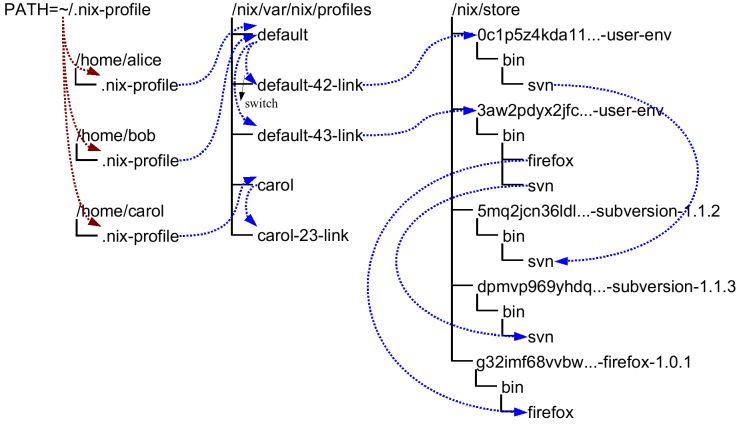
\includegraphics[width=0.85\textwidth]{thesis/graphics/nix-user-environments.png}
  \caption{Directory tree of symlinks in the Nix store (\texttt{/nix/store}) that define the active packages (and their dependencies) of a user environment \cite{Profiles}.}
  \label{fig:nix-user-environments}
\end{figure}

\subsection{Package management}\label{nix-tools-package-management}
Nix provides a collection of Nix expressions, called the \emph{Nix package collection} (Nixpkgs), which is a git repository that contains packages as Nix expressions ranging from build tools like \verb|GCC| and \verb|Glibc| to user applications like Mozilla Firefox. It is possible to write one's own package collection or extend Nixpkgs. To easily stay up to date with new versions of Nixpkgs, we can use the \emph{Nix channel} mechanism \cite{NixPackageManagement}. A nix-channel is a name for the latest ``verified'' commits in Nixpkgs, where ``verified'' is defined on a channel basis. These channels provide binary builds of packages that are cached in the Nix binary cache. One can, for example, add different channels and switch between them on a user-level basis \cite{NixChannels}.

\subsection{User environments and multi-user mode}\label{Nix-multi-user}
In Nix, \emph{user environments} allow atomic updates, atomic rollbacks, and users to have custom configurations. Different users may ``see'' different subsets of the set of all installed applications on the system. This subset is specified in a directory in the user's \verb|PATH| and is called a user environment \cite{NixIntroduction}. 
Nix uses a directory tree of symlinks inside the Nix store depicted in figure \ref{fig:nix-user-environments} to achieve the linking between user environments (\path{/nix/store/0c1p5z4...-user-env}) and the active packages (e.g. \verb|subversion-1.1.2|) they use. The discussion of Nix profiles is out of the scope of this work \cite{Profiles}. %\emph{Generations} outside the store (e.g. \verb|default-42-link|) point to user environments. A new generation is created by each \verb|nix-env| operation (i.e., when installing new packages or changing the profile) and is based on the current one. Generations are grouped into profiles so that users do not interfere with each other \cite{Profiles}.

Nix has a multi-user mode that allows multiple users to safely share a Nix store by ensuring that users cannot arbitrarily run builders that modify the Nix store or database or interfere with other users' builds. User-space limitations achieve this: the Nix store and database are owned by a privileged user, and builders are executed under special user accounts. If an unprivileged user runs a Nix command, then actions that operate on the Nix store are performed by the \emph{Nix daemon} running as the owner of the Nix store \cite{NixMultiUser}. 

\subsection{The \textbf{\texttt{nix-shell}} and \textbf{\texttt{nix-build}} commands}\label{nix-shell&nix-build}
The \verb|nix-shell| command helps reproduce a development environment for a package without building the derivation \cite{NixIntroduction}\cite{NixShell}. Given a Nix expression, the command \verb|nix-shell| constructs an isolated environment with all the inputs needed to run the build script but does not execute the build script as the \verb|nix-build| command. To this end, \verb|nix-shell| builds the dependencies of the expression from the source or downloads them from a binary cache if they are not already in the Nix store. It will then source a setup script that sets all necessary environment variables (e.g., the \verb|PATH|, compiler search path, Nix profile) to their corresponding values. After that, the command starts a shell in which all the environment variables are set.

In short, the \verb|nix-shell| command only sets up a development environment from the expression without building a new derivation. We use the \verb|nix-build| command to build new derivations from an expression. 

\subsection{Nix functions for Docker compatible images}\label{nix-dockertools}
Nix provides a set of functions (\verb|dockerTools|) for creating and manipulating container images. These functions do not need Docker itself for their operations. %The \verb|buildImage| function builds a Docker-compatible tarball containing a single image with multiple layers. 
The \verb|buildLayeredImage| function builds an image with many of the store paths on their own layer, and each is realized as a tarball. The \verb|streamLayeredImage| function streams an uncompressed tarball of an image to \verb|stdout|, which avoids realizing the image into the Nix store, therefore saving on I/O operations and disk/cache space \cite{DockerTools}. Both commands' tarball(s) can be loaded into Docker or pushed to a registry.